\documentclass{scrreprt}
\usepackage{listings}
\usepackage{underscore}
\usepackage{graphicx}
\usepackage[bookmarks=true]{hyperref}
\usepackage[utf8]{inputenc}
\usepackage[english]{babel}
\usepackage[utf8]{inputenc}
\usepackage[T2A]{fontenc}% Required for inserting images
\usepackage[left=2cm,right=2cm,
    top=1cm,bottom=1cm,bindingoffset=0cm]{geometry}
\hypersetup{
    bookmarks=false,    % show bookmarks bar?
    pdftitle={Software Requirement Specification},    % title
    pdfauthor={Jean-Philippe Eisenbarth},                     % author
    pdfsubject={TeX and LaTeX},                        % subject of the document
    pdfkeywords={TeX, LaTeX, graphics, images}, % list of keywords
    colorlinks=true,       % false: boxed links; true: colored links
    linkcolor=blue,       % color of internal links
    citecolor=black,       % color of links to bibliography
    filecolor=black,        % color of file links
    urlcolor=purple,        % color of external links
    linktoc=page            % only page is linked
}%
\def\myversion{1.0 }
\date{}
%\title
\usepackage{hyperref}
\begin{document}

\begin{flushright}
    \rule{16cm}{5pt}\vskip1cm
    \begin{bfseries}
        \Huge{SOFTWARE REQUIREMENTS\\ SPECIFICATION}\\
        \vspace{1.5cm}
        for\\
        \vspace{1.5cm}
        TELEGRAM BOT - GETCOURT\\
        \vspace{1.5cm}
        \LARGE{Version \myversion}\\
        \vspace{1.5cm}
        Prepared by : Todorov Denis\\
        \vspace{1.5cm}
        Submitted to : Andrey Ivanov \\Lecturer\\
        \vspace{1.5cm}
        \today\\
    \end{bfseries}
\end{flushright}

\tableofcontents

\chapter{Introduction}

\section{Purpose}
Целью данного Telegram бота 'GetCourt' является предоставление пользователю возможности находить партнеров для занятия спортом и места для игры в командные виды спорта. Я создаю это приложение, чтобы помочь решить проблему одиночной игры и предоставить спортсменам удобный способ находить партнеров для занятий спортом и места для проведения мероприятий.

\section{Document conventions}
API (Application programming interface) – это контракт, который предоставляет программа. «Ко мне можно обращаться так и так, я обязуюсь делать то и это».
GitHub – это облачная платформа для хостинга IT-проектов и совместной разработки, под капотом которой находится популярная система контроля версий Git, а также полноценная социальная сеть для разработчиков.
Паттерн программирования – образец, шаблон. В программировании это понятие подразумевает использование определенного подхода или алгоритма, который уже существует для решения проблемы в той или иной ситуации.
Фреймворк – готовая модель в IT, заготовка, шаблон для программной платформы, на основе которого можно дописать собственный код.
GIL (Global Interpreter Lock) – глобальная блокировка интерпретатора в Python, накладывающая некоторые ограничения на потоки.
Деплой – это развертывание и запуск веб-приложения, сайта или бота в его рабочей среде, то есть на сервере или хостинге. Разработчик загружает приложение, написанное на локальном компьютере, в специальное пространство, из которого оно доступно в интернете.
Хендлер – это обработчик запросов от пользователя.
База данных (БД) – это упорядоченный набор структурированной информации или данных, которые обычно хранятся в электронном виде в компьютерной системе. База данных обычно управляется системой управления базами данных (СУБД).



\section{Intended Audience and Reading Suggestions}
This SRS is for developers, project managers, users and testers. Further the discussion will provide all the internal, external, functional and also non-functional informations about "GetCourt".
\newline
\begin{figure}
    \centering
    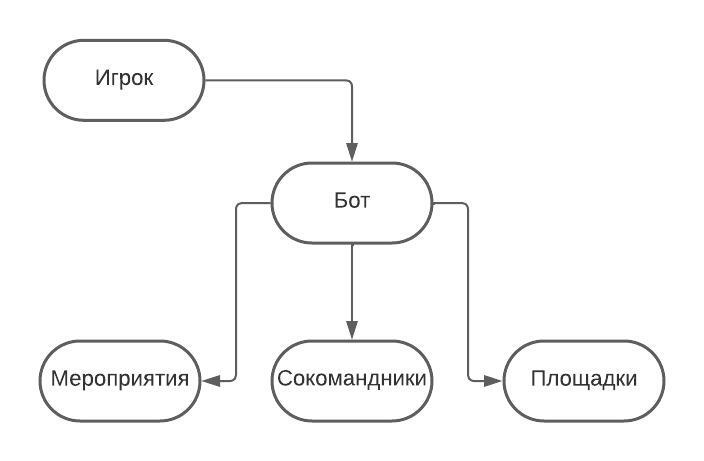
\includegraphics[width=10cm]{project scope.jpeg}
    \caption{Entire work-flow}
    \label{fig:IICT WEBSITE}
\end{figure}
\newline
Figure 1.1 (Entire work-flow) is the overview of the project. Connection of all the entities are dependable to each others.  This gives the simple idea about the functional activities of the project. 
\newline


\section{References}

[1] Async IO in Python: A Complete Walkthrough
(https://realpython.com/async-io-python/)
\newline
[2] Getting Started With Async Features in Python
(https://realpython.com/python-async-features/)
\newline
[3] AsyncIOTelegram sendlocation (https://docs.aiogram.dev/uk_UA/latest/api/methods/send_location.html)
\newline
[4] SQlite library
(https://blog.skillfactory.ru/glossary/sqlite/)
\newline
[5]  GeoPy
(https://geopy.readthedocs.io/en/stable/)
\newline
[6] Haversine Distance Equation
(https://medium.com/analytics-vidhya/finding-nearest-pair-of-latitude-and-longitude-match-using-python-ce50d62af546/)
\newline
[7] SQL
(https://www.w3schools.com/sql/)

\chapter{Overall Description}

\section{Product Perspective}
Целью проекта является создание Telegram-бота "СпортПартнер", который поможет пользователям находить партнеров и площадки для командных видов спорта.

\section{Product Features}
Продукт будет включать в себя следующие функции:
\newline
Выбор вида спорта: Пользователь может выбрать вид спорта, который его интересует.
\newline
Поиск ближайшей площадки: Пользователь может найти ближайшую площадку для выбранного вида спорта на основе своей геолокации.
\newline
Добавление площадки: Пользователь может добавить площадку с фотографиями, описанием и информацией о уровне игроков.
\newline
Создание мероприятия: Пользователь может создать мероприятие для выбранного вида спорта.
\newline
Регистрация на мероприятие: Пользователь может зарегистрироваться на мероприятие, созданное другим пользователем.
\newline
Опциональная регистрация: Пользователь может создать профиль с фотографией, описанием, уровнем игры и социальными сетями.
\newline
Личный кабинет: У каждого пользователя есть личный кабинет для управления своей активностью.

\section{User Classes and Characteristics}
\begin{figure}
    \centering
    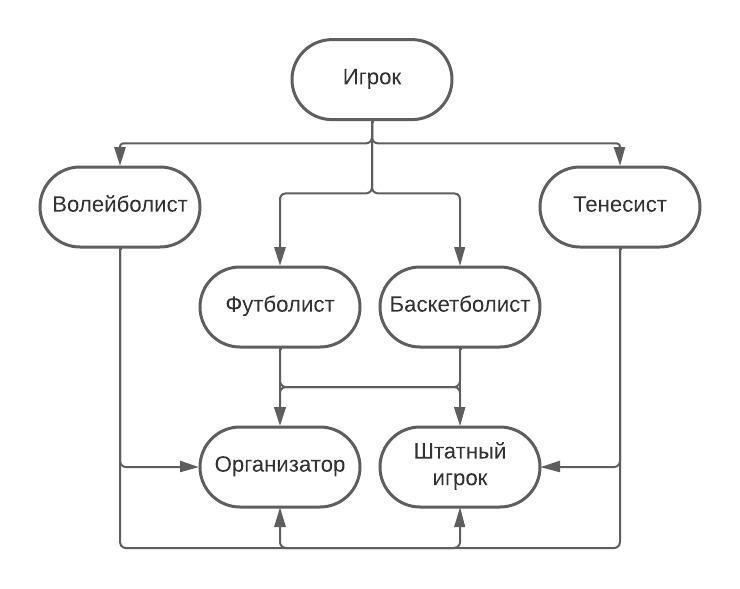
\includegraphics[width=8cm]{project scope (1).jpeg}
    \caption{type of users}
    \label{fig:type of users}
\end{figure}

\pagebreak

\section{Product Functions}

\begin{figure}[h!]
    \centering
    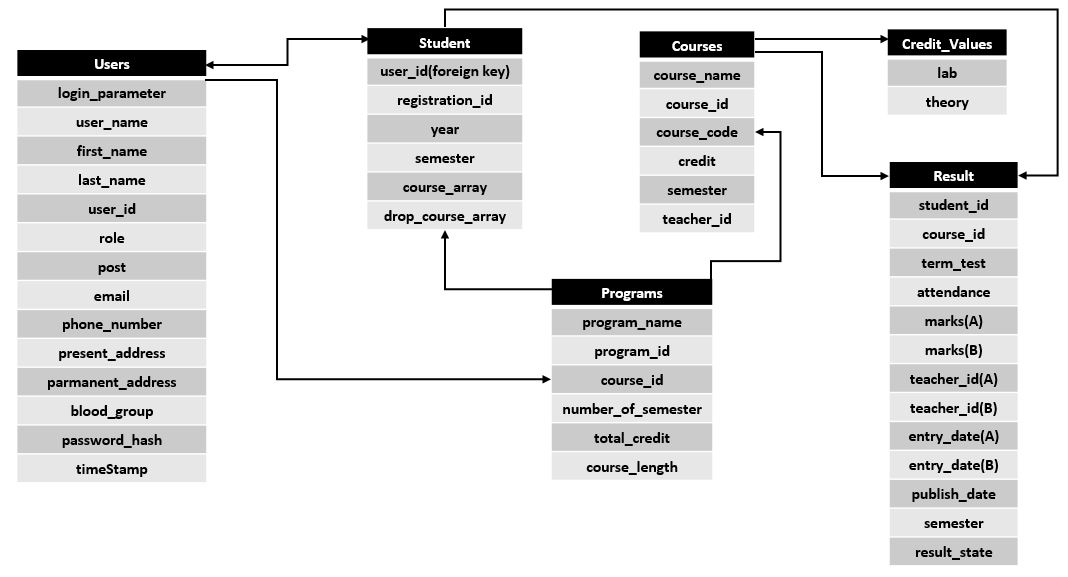
\includegraphics[width=15cm]{3.JPG}
    \caption{Data Flow Diagram}
    \label{fig:Data Flow Diagram}
\end{figure}


\section{Operating Environment}
Система будет работать в Telegram Messenger и будет использовать геолокацию для определения местоположения пользователя.

\section{Design and Implementation constraints}
Система должна соответствовать стандартам и ограничениям Telegram API. Для хранения данных предполагается использовать реляционную базу данных.
\begin{itemize}
    \item Python 3.11
    \item PosstgreSQL 15
    \item UTF 8
    \item Telegram API
\end{itemize}


\section{User documentation}
Docs for user-flow

\section{Assumptions and Dependencies}
\begin{itemize}
    \item Aiogram 3.1.1
    \item AsyncIO 3.4.3
\end{itemize}

\chapter{System Features}
Результатом моего Телеграм бота является утилита, которая позволяет загружать данные и выгружать для пользовательского использования.

\section{Выбор вида спорта}

\subsection{Description and Priority}
Пользователь может выбрать один из доступных видов спорта, таких как футбол, баскетбол, волейбол, и другие.
\newline
\textbf{Приоритет:} высокий

\subsection{Stimulus/Response sequences}
\begin{itemize}
    \item Стимул: Пользователь запускает бота.
    \item Реакция: Бот отображает список доступных видов спорта и предлагает пользователю выбрать один.
\end{itemize}

\subsection{Functional Requirements}
\begin{itemize}
    \item Бот должен предоставлять список доступных видов спорта.
    \item Пользователь должен иметь возможность выбрать один вид спорта.
\end{itemize}

\section{Поиск ближайшей площадки}

\subsection{Description and Priority}
Пользователь может найти ближайшую площадку для выбранного вида спорта на основе своей геолокации.
\newline
\textbf{Приоритет:} высокий

\subsection{Stimulus/Response sequences}
\begin{itemize}
    \item Стимул: Пользователь выбирает вид спорта и запрашивает поиск площадки.
    \item Реакция: Бот использует геолокацию пользователя и находит ближайшую площадку.
\end{itemize}

\subsection{Functional Requirements}
\begin{itemize}
    \item Бот должен иметь доступ к геолокации пользователя.
    \item Бот должен иметь доступ к базе данных площадок.
    \item Бот должен позволить пользователю выбирать вид спорта и выполнять поиск площадки.
    \item Бот должен отобразить результаты поиска, включая информацию о ближайших площадках.
\end{itemize}



\section{Добавление площадки}

\subsection{Description and Priority}
Пользователь может добавить информацию о новой площадке для выбранного вида спорта, включая фотографии, описание и уровень игроков.
\newline
\textbf{Приоритет:} средний

\subsection{Stimulus/Response sequences}
\begin{itemize}
    \item Стимул: Пользователь выбирает опцию "Добавить площадку".
    \item Реакция: Бот запрашивает информацию о площадке и фотографии.
\end{itemize}

\subsection{Functional Requirements}
\begin{itemize}
    \item Бот должен предоставить опцию для добавления новой площадки.
    \item Пользователь должен иметь возможность ввести информацию о площадке, такую как название, описание, уровень игроков, и загрузить фотографии.
    \item Бот должен хранить информацию о добавленных площадках в базе данных.
\end{itemize}

\section{Создание мероприятия}

\subsection{Description and Priority}
Пользователь может создать мероприятие для выбранного вида спорта, устанавливая дату, время и местоположение.
\newline
\textbf{Приоритет:} средний

\subsection{Stimulus/Response sequences}
\begin{itemize}
    \item Стимул: Пользователь выбирает опцию "Создать мероприятие".
    \item Реакция: Бот запрашивает информацию о мероприятии, включая дату, время и местоположение.
\end{itemize}

\subsection{Functional Requirements}
\begin{itemize}
    \item Бот должен предоставлять опцию для создания мероприятия.
    \item Пользователь должен иметь возможность ввести информацию о мероприятии, такую как дата, время, местоположение и описание.
    \item Бот должен хранить информацию о созданных мероприятиях в базе данных.
\end{itemize}

\section{Регистрация на мероприятие}

\subsection{Description and Priority}
Пользователь может зарегистрироваться на мероприятие, созданное другим пользователем, для участия.
\newline
\textbf{Приоритет:} средний

\subsection{Stimulus/Response sequences}
\begin{itemize}
    \item Стимул: Пользователь выбирает мероприятие и опцию "Зарегистрироваться".
    \item Реакция: Бот регистрирует пользователя на мероприятие.
\end{itemize}

\subsection{Functional Requirements}
\begin{itemize}
    \item Бот должен отображать список доступных мероприятий.
    \item Пользователь должен иметь возможность выбрать мероприятие и зарегистрироваться на него.
    \item Бот должен уведомлять о регистрации на мероприятие.
\end{itemize}

\section{Опциональная регистрация}

\subsection{Description and Priority}
Пользователь может создать профиль с дополнительной информацией, такой как фото, описание, уровень игры и ссылки на социальные сети.
\newline
\textbf{Приоритет:} низкий

\subsection{Stimulus/Response sequences}
\begin{itemize}
    \item Стимул: Пользователь выбирает опцию "Зарегистрироваться".
    \item Реакция: Бот запрашивает дополнительную информацию для профиля.
\end{itemize}

\subsection{Functional Requirements}
\begin{itemize}
    \item Бот должен предоставлять опцию для опциональной регистрации.
    \item Пользователь может ввести информацию о себе, такую как фотография, описание, уровень игры и ссылки на социальные сети.
    \item Бот должен хранить информацию о пользователях в базе данных.
\end{itemize}

\section{Личный кабинет}

\subsection{Description and Priority}
Каждый пользователь должен иметь доступ к личному кабинету для управления своей активностью и информацией.
\newline
\textbf{Приоритет:} низкий

\subsection{Stimulus/Response sequences}
\begin{itemize}
    \item Стимул: Пользователь выбирает опцию "Личный кабинет" для того, чтобы увидеть надавние площадки, на которых он играл и не искать заново.
    \item Реакция: Бот предоставляет информацию о личных данных, приобретенных в процессе и использования бота.
\end{itemize}

\subsection{Functional Requirements}
\begin{itemize}
    \item Бот должен предоставлять каждому пользователю личный кабинет.
    \item Пользователь должен иметь возможность просматривать и редактировать свой профиль, а также управлять своими созданными мероприятиями и площадками.
\end{itemize}


\chapter{External interface requirements}

\section{User interfaces}
Бот должен предоставлять простой и интуитивно понятный пользовательский интерфейс для взаимодействия с пользователями.
\begin{itemize}
    \item Интерфейс должен быть легко понятен и доступен для пользователей всех уровней опыта.
    \item Интерфейс должен включать элементы управления для выбора видов спорта, поиска площадок, создания мероприятий и других функций.
\end{itemize}

\section{Software interfaces}
Разраб/Админ должен иметь интерфейс для управления пользователями, мероприятиями и площадками(всем функционалом).
\begin{itemize}
    \item Разраб/Администратор должен иметь доступ к интерфейсу управления, где он может блокировать пользователей, удалять мероприятия и площадки, а также выполнять другие административные функции.
\end{itemize}

\section{Hardware interfaces}
something

\section{Communication interfaces}
something

\chapter{Non functional requirements}

\section{Performance Requirements}

\section{Требования к производительности}

\subsection{Отклик системы}
Бот должен быстро реагировать на запросы пользователей и обеспечивать плавное взаимодействие.
\begin{itemize}
    \item Время отклика бота на запросы пользователя не должно превышать 2 секунды.
\end{itemize}

\subsection{Пропускная способность}
Система должна обеспечивать высокую пропускную способность для обработки множества пользователей и данных.
\begin{itemize}
    \item Система должна поддерживать не менее 10 000 активных пользователей одновременно.
\end{itemize}

\section{Security Requirements}
No one without registered users can inter to the website. One particular user of a section only can perform his/her particular actions.

\subsection{Защита данных}
Система должна обеспечивать защиту данных пользователей и их личной информации.
\begin{itemize}
    \item Данные пользователей должны храниться в зашифрованной форме.
    \item Доступ к базе данных должен быть ограничен и защищен от несанкционированного доступа.
\end{itemize}

\section{Software Quality Attributes}
In the development phase also testing and conferences of users is been continued. So that the quality of the software is been maintained and all the requirements are been fulfilled.

\subsection{Тестирование}
Программное обеспечение должно быть подвергнуто тестированию, чтобы обнаружить и исправить ошибки.
\begin{itemize}
    \item Перед выпуском в продакшен, бот должен пройти тестирование, включая модульное, интеграционное и системное тестирование.
\end{itemize}

\subsection{Обновления и поддержка}
После выпуска MVP, разработка и поддержка бота должны быть продолжены для внесения улучшений и исправлений.
\begin{itemize}
    \item Команда разработки должна регулярно выпускать обновления для бота.
    \item Поддержка и обновления должны предоставляться в течение не менее 12 месяцев после выпуска MVP.
\end{itemize}

\section{Business Rules}

\subsection{Расширяемость}
Система должна быть разработана с учетом возможности расширения и добавления новых видов спорта и функций в будущем.
\begin{itemize}
    \item Архитектура системы должна быть модульной и легко расширяемой.
\end{itemize}

\chapter{Other Requirements}

\section{Appendix A: Glossary}

\section{Appendix B: Analysis Models}

\section{Appendix C: Issues list}

\end{document}